\section{Overview}
\label{sec:overview}

We give a tour of ILC and SaUCy (explaining the universal composability
framework en route) with a simple example: How can two untrusting parties, Alice
and Bob, securely flip a coin? (The answer: a commitment scheme.)

\begin{figure*}[t]
\centering
\begin{tabular}{c|c}
\begin{subfigure}{.575\textwidth}
    $\Func_{\textsc{com}}$ proceeds as follows, running with parties $A$ and
  $B$.
    \begin{enumerate}
        \item Upon receiving a message $(\mathsf{Commit}, b)$ from $A$, where $b
          \in \{ 0, 1 \}$, record the value $b$ and send the message
          $(\mathsf{Receipt})$ to $B$. Ignore any subsequent \textsf{Commit}
          messages.
        \item Upon receiving a message $(\mathsf{Open})$ from $A$, proceed as
          follows: If some value $b$ was previously recorded, then send the
          message $(\mathsf{Open}, b)$ to $B$ and halt. Otherwise, halt.
    \end{enumerate}
\label{func:com}
\end{subfigure}\hspace{0.02\textwidth}
&\hspace{0.02\textwidth}
\begin{subfigure}{.35\textwidth}
  \lstinputlisting[style=myilc]{listings/Fcom.ilc}
\end{subfigure}
\end{tabular}
\caption{An ideal functionality for a one-time commitment scheme in prose (left)
  and in ILC (right).}
\label{func:com}
\end{figure*}

\subsection{Ideal Functionalities}
\label{subsec:functionalities}

Security in the UC framework is based on the real/ideal
paradigm~\cite{goldreich1987play}. To carry out some cryptographic task in the
real world, a set of parties must execute a protocol for the task among
themselves in a distributed fashion. In the ideal world, however, the parties
securely access an \emph{ideal functionality} $\mc{F}$, which is imagined as an
incorruptible trusted third party that securely (by construction) carries out
the task to be achieved by the protocol. To do so, $\mc{F}$ obtains inputs from
the parties, performs some local computation, and hands outputs back to the
parties. Because $\mc{F}$ is trivially secure, it serves as a uniform way to
describe the task's security requirements.\smallskip

\myheader{Example: Secure coin flipping.} Suppose two untrusting parties, Alice
and Bob, wish to securely flip a coin---Alice calls the coin flip by publishing a
bit $b \in \{ 0, 1\}$, and Bob flips the coin by publishing the result $r \in \{0,
1\}$. If $b = r$, then Alice wins; otherwise, Bob wins. Observe that simply
having Alice and Bob publish their respective values is not secure. If Alice
publishes $b$ first, then Bob can cheat by manipulating $r$ in his favor (and
vice versa)!

In order to carry out the coin flip securely, they can use a commitment
scheme~\cite{brassard1988minimum}, which has the following interaction:
\begin{enumerate}[leftmargin=*]
\item Alice: Commit to $b$ as $C = \mathsf{com}(b)$, and send $C$ to Bob.
\item Bob: Compute and send the result $r$ to Alice.
\item Alice: Open the commitment as $b' = \mathsf{open}(C)$, and send it to Bob.
\end{enumerate}
\noindent If $r = b'$, then Alice wins; otherwise, Bob wins. But what is to stop
either party from cheating? In order for the protocol to be secure, it should
satisfy these important properties (stated informally):
\begin{itemize}[leftmargin=*]
  \item \emph{Hiding.} The commitment $C$ should hide $b$ from Bob, so that he
    cannot manipulate $r$ in his favor.
  \item \emph{Binding.} It should be the case that $b =
    \mathsf{open}(\mathsf{com}(b))$, so that Alice cannot open to a different
    value.
  \item \emph{Non-malleability.} \todo{Also needs this?}
\end{itemize}

\myheader{Commitment functionality.} We can capture both the hiding and binding
properties at once by defining an ideal functionality $\Func_{\textsc{com}}$ for
a (one-time) commitment scheme as it would appear in the cryptography literature
(Figure~\ref{func:com}, left).

Upon receiving the bit $b$ that Alice wishes to commits to,
$\Func_{\textsc{com}}$ records $b$ and notifies Bob that it has done so. Then,
whenever Alice wants to reveal $b$ to Bob, she notifies $\Func_{\textsc{com}}$,
which sends it to Bob. Because, in this idealized world, Alice and Bob trust
$\Func_{\textsc{com}}$ to do all the work, the hiding and binding properties
hold trivially. Of course, in the real world, Alice and Bob would not want to
trust such a third party (if it even exists), so their hope is that the
commitment scheme they use is ``just as good as''
$\Func_{\textsc{com}}$.\smallskip

\subsection{ILC By Example}
\label{subsec:ilc-flavored}

In Figure~\ref{func:com} (right), we have written $\Func_{\textsc{com}}$ in ILC,
which we use to highlight the key features of the language. \todo{Update example
  to eliminate irrefutable pattern matches.}\smallskip

\myheader{Linear types.} Let us first examine the function signature of
\textsf{fCom}, which (glossing over some details) takes as arguments two
channels, a read channel \textsf{frA} and a write channel \textsf{toB}, and
returns \textsf{Unit}. There are a number of things to unpack here:

\begin{itemize}[leftmargin=*]
  \item The signature consists of linear arrows $\multimap$ (or ``lollipops''), which
    describe the types of linear functions that consume their argument exactly
    once.
  \item A function arrow (both linear and intuitionistic) carries the modal type
    (either $\Wm$, $\Rm$, or $\Vm$) of its function body. In the example, the
    left lollipop has mode $\Vm$, which we elide, and the right lollipop has
    mode $\Rm$. We have more to say about modes later.
  \item Channels are typed. Both \textsf{frA} and \textsf{toB} communicate
    values inhabiting the sum type \textsf{Msg}.
  \item Read channels are linearly typed to protect them from duplication. This
    ensures that no confusion arises as to which process is being written to.
  \item Write channels and the unit value are intuitionistically typed. Hence,
    their types require the ! operator (pronounced ``bang!''), which lifts an
    intuitionistic type into a linear type.
\end{itemize}

\noindent ILC achieves the above with a two-kind system. That is, types are
bifurcated into a kind for intuitionistic types and a kind for linear
types.\smallskip

\myheader{Modal types.} ILC expressions are also typed with one of three modes:
$\Wm$ (write mode), $\Rm$ (read mode), or $\Vm$ (value mode). Modes can be
composed either sequentially or in parallel to yield new modes.

To give a few examples, suppose expressions $e_1$ and $e_2$ have modes $m_1$ and
$m_2$, respectively. Sequential mode composition shows up in the obvious case of
sequentially evaluating the two expressions, so the mode of $\eSeq{e_1}{e_2}$ is
$m1 ;; m2 => m3$. Parallel mode composition shows up when one process forks a
second process, so the mode of $\eFork{e_1}{e_2}$ is $m_1 || m_2 =>
m_3$. \todo{Explain fork.}

The rules for mode composition are fleshed out in Section~\ref{sec:ilc}, but the
key takeaway here is that composing write mode processes in parallel is
\emph{not allowed}. That is, $\Wm || \Wm => p$ is not derivable for any mode
$p$. Recall that in the ITM model, execution is essentially single-threaded, so
this ensures that no confusion arises as to which process is currently writing,
or equivalently, which process is currently active. A program violating this
invariant would not be expressible as ITMs.\smallskip

\myheader{Putting it all together.} The function body of \textsf{fCom} closely
follows $\Func_{\textsc{com}}$, but there are several points worth mentioning.
First, we introduce the letrd and wr typing rules for read and write
expressions. Typing judgements have the form $\Delta ; \Gamma |- e : A |> m$, where $\Delta$ is
a linear typing context, $\Gamma$ is an intuitionistic typing context, and $m$ is a
mode.
\begin{mathpar}
\Infer{letrd}
{\Delta_1 ; \Gamma |- e_1 : \tyRd{A}\\
\Delta_2,x_1:\tyBang{A},x_2:\tyRd{A} ; \Gamma |- e_2 : B |> m
}
{\Delta_1, \Delta_2 ; \Gamma |- \eLetRd{x_1}{x_2}{e_1}{e_2} : B |> \Rm}
\end{mathpar}

The letrd rule says that if we can partition the linear context $\Delta$ as $\Delta_1,
\Delta_2$ such that $e_1$ has type $\tyRd{A}$ and mode $\Vm$ (elided) under contexts
$\Delta_1; \Gamma$ and $e_2$ has type $B$ and mode $m$ under contexts
$\Delta_2,x_1:\tyBang{A},x_2:\tyRd{A} ; \Gamma$, then the full expression has type $B$ and
mode $\Rm$. Notice several things:
\begin{itemize}[leftmargin=*]
  \item Reading on channel of type $\tyRd{A}$ produces a linear pair (or
    ``tensor'') of type $\tyTensor{\tyBang{A}}{\tyRd{A}}$.
  \item ILC only allows intuitionistically typed values to be sent over channels
    ($A$ ranges over intuitionistic types), so the value read on the channel is
    lifted into the first element of the tensor as a linear type.
  \item The read channel itself is returned as the second tensor element, so
    that it may be rebound and used again.
  \item In \textsf{fCom}, pattern matching with the ! operator unpacks linear
    values, so the value bound to $b$ in the first read from \textsf{frA} has an
    intuitionistic type.
\end{itemize}
\begin{mathpar}
\Infer{wr}
{\Delta_1; \Gamma   |- e_1 : A\\
\Delta_2; \Gamma   |- e_2 : \tyWr{A}}
{\Delta_1, \Delta_2; \Gamma |- \eWr{e_1}{e_2} : \tyUnit |> \Wm}
\end{mathpar}

The wr rule says that if we can partition the linear context $\Delta$ as $\Delta_1, \Delta_2$
such that $e_1$ has type $A$ and mode $\Vm$ and $e_2$ has a type $\tyWr{A}$ and
mode $\Vm$, then the full expression has type $\tyUnit$ and mode $\Wm$.

Revisiting \textsf{fCom}, the two letrd expressions are composed sequentially,
so the mode of the entire function body is derived as $\Rm ;; \Rm => \Rm$
according to our mode composition rules. This is reflected in the fact that the
right lollipop in the function signature carries a mode $\Rm$. Finally, because
wr expressions return $\eUnit$, we wrap it inside a bang! to lift its type into
the linear type \textsf{!Unit}.

\subsection{UC Emulation}
\label{subsec:emulation}

Having defined security in the form of an ideal functionality, the next step is
to prove that a protocol meets the definition. We say that a protocol $\pi$
\emph{emulates} (or \emph{securely realizes}) an ideal functionality $\mc{F}$ if
every adversarial behavior in the real world (running with $\pi$) can also be
exhibited in the ideal world (running with $\mc{F}$). But because $\mc{F}$ is
secure by construction, whatever adversarial behavior can take place in the
ideal world does not lead to a break in security.

Proving emulation formally proceeds in two steps:
\begin{enumerate}[leftmargin=*]
\item The first step is constructive: We must construct a \emph{simulator}
  $\mc{S}$ (a simulated adversary) that can emulate the attack of any adversary
  $\mc{A}$ on $\pi$, but instead, on $\mc{F}$.
\item The second step is a relational analysis: We must show that running $\pi$
  under attack by any adversary $\mc{A}$ (the real world) is
  \emph{indistinguishable} from running $\mc{F}$ under attack by $\mc{S}$ (the
  ideal world) to any distinguisher $\mc{Z}$, called the \emph{environment}.
\end{enumerate}
In particular, $\mc{Z}$ is an interactive distinguisher: It interacts with the
real world and the ideal world in a well-defined manner, and the simulation is
good if no $\mc{Z}$ can distinguish between the two. We call this game the UC
experiment.

\begin{figure}
  \centering
  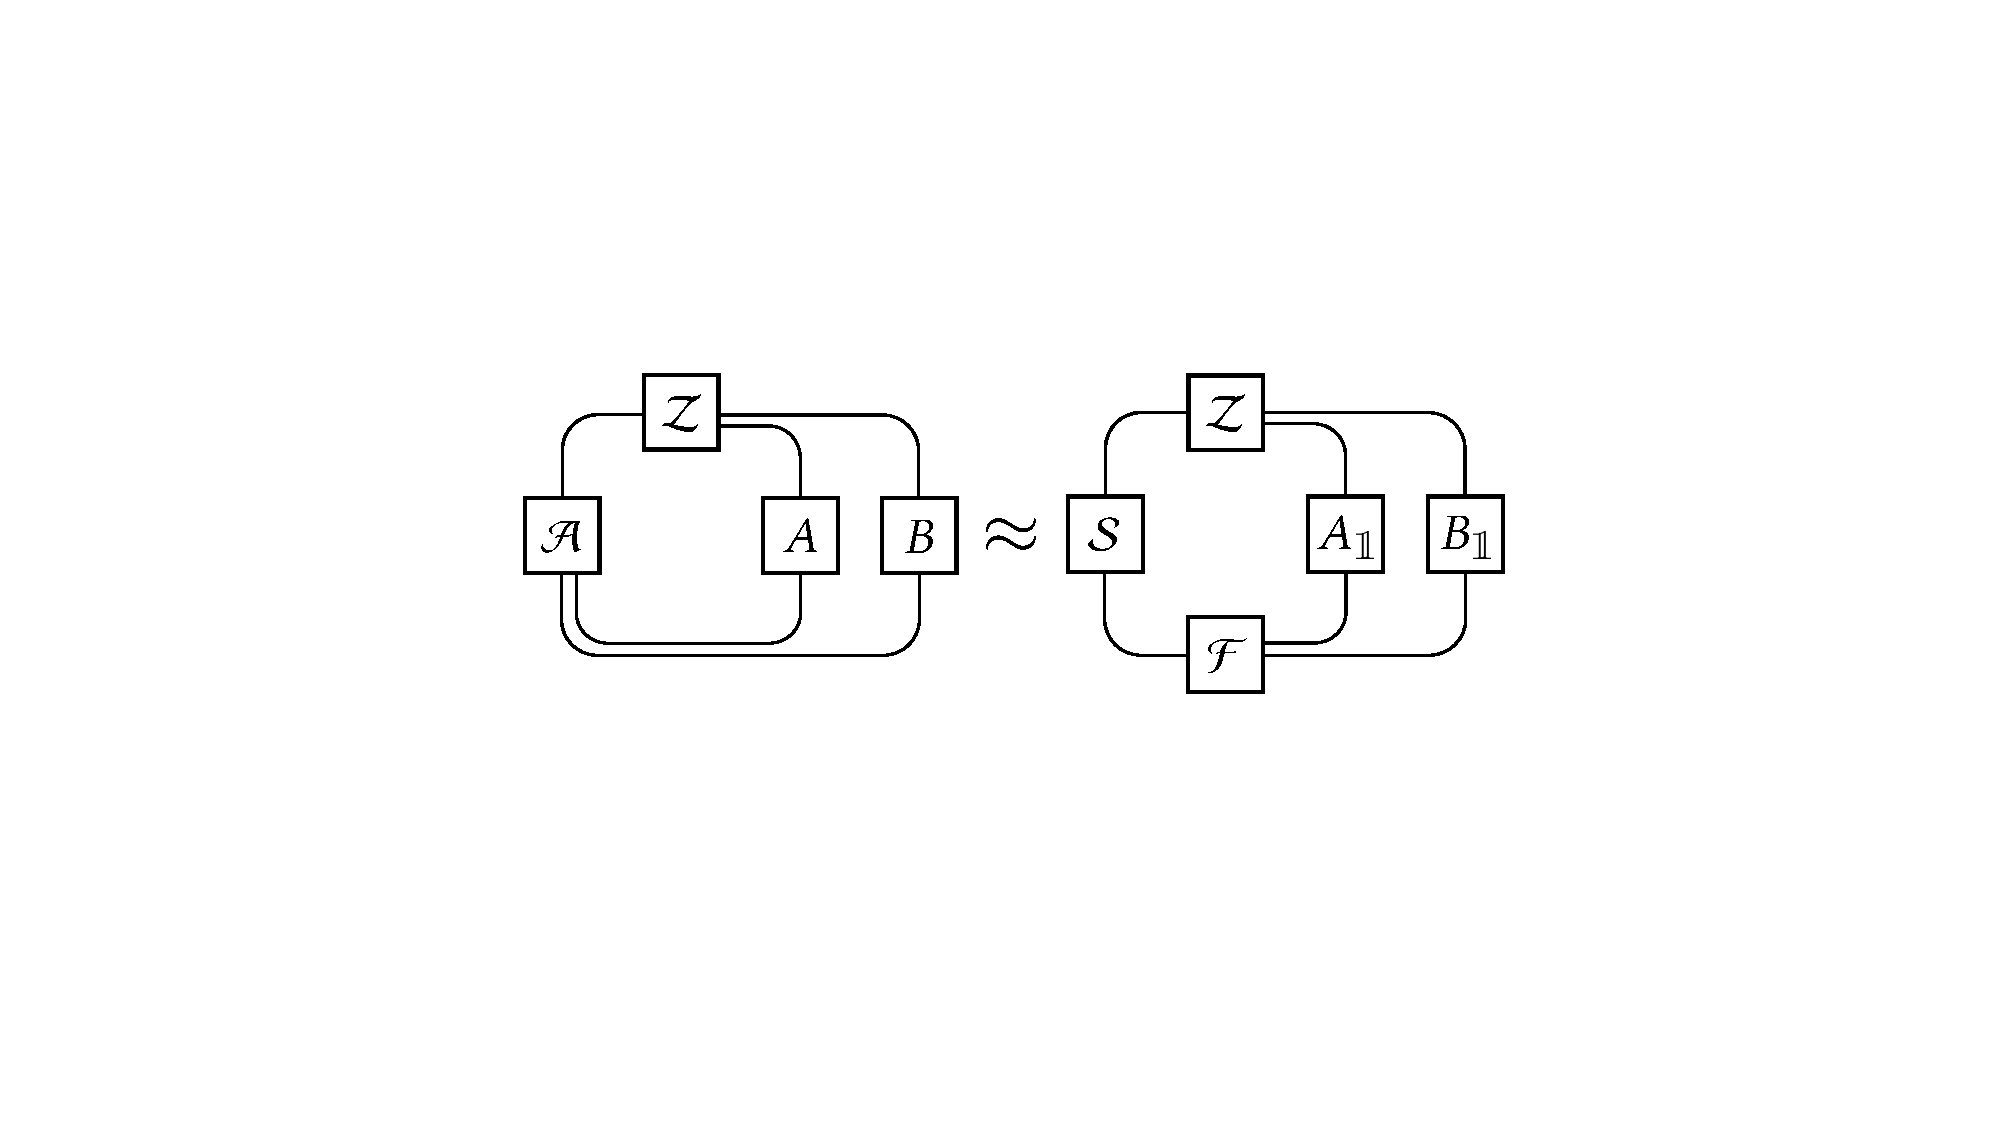
\includegraphics[width=0.85\linewidth]{graphics/suc-experiment}
  \caption{UC experiment with real world (left) and ideal world (right).}
  \label{fig:uc-experiment}
\end{figure}

\todo{Need to make this paragraph more clear.} Figure~\ref{fig:uc-experiment}
illustrates the UC experiment in the context of the commitment scheme defined
previously. The real world is shown on the left and the ideal world is shown on
the right, with connecting lines denoting communication channels.\footnote{Note
  that in the real world, all communication passes through the adversary
  $\mc{A}$. In the bare model, communication is asynchronous, unauthenticated,
  and unreliable, but other models of communication can be built atop this
  model.} In the real world, $A$ and $B$ carry out the protocol with eachother,
while in the ideal world, $A$ and $B$ are ``dummy'' parties that simply relay
messages between $\mc{Z}$ and $\mc{F}$. The environment $\mc{Z}$ is tasked to
interact with each world and distinguish between the two.

\subsection{A Flavor of SaUCy}
\label{subsec:sauce-flavored}

\todo{SaUCy prelude, UC metatheory}

\begin{comment}
\subsection{UC composition}
\label{subsec:composition}

The advantage of security definitions in UC is that they satisfy strong
composability guarantees, even under concurrent composition. Suppose that $\pi_1$
is a protocol that securely realizes a functionality $\mc{F}_1$. If a protocol
$\pi_2$, using $\mc{F}_1$ as a subroutine, securely realizes a functionality
$\mc{F}_2$, then the protocol $[\pi_1 / \mc{F}_1]\pi_2$, in which calls to
$\mc{F}_1$ are replaced by calls to $\pi_1$, also securely realizes
$\mc{F}_2$. That way, it suffices to analyze the security of the standalone
protocol $\pi_2$ in the $\mc{F}_1$-hybrid model, where parties run $\pi_2$ with
access to $\mc{F}_1$, as opposed to the composite protocol of $\pi_2$ and
$\pi_1$. Figure~\ref{fig:uc-composition} illustrates protocol composition. The
setup on the left represents the $\mc{F}_1$-hybrid model, and the setup on the
right represents the protocol substitution $[\pi_1 / \mc{F}_1]\pi_2$, which
maintains security.

\begin{figure}
  \centering
  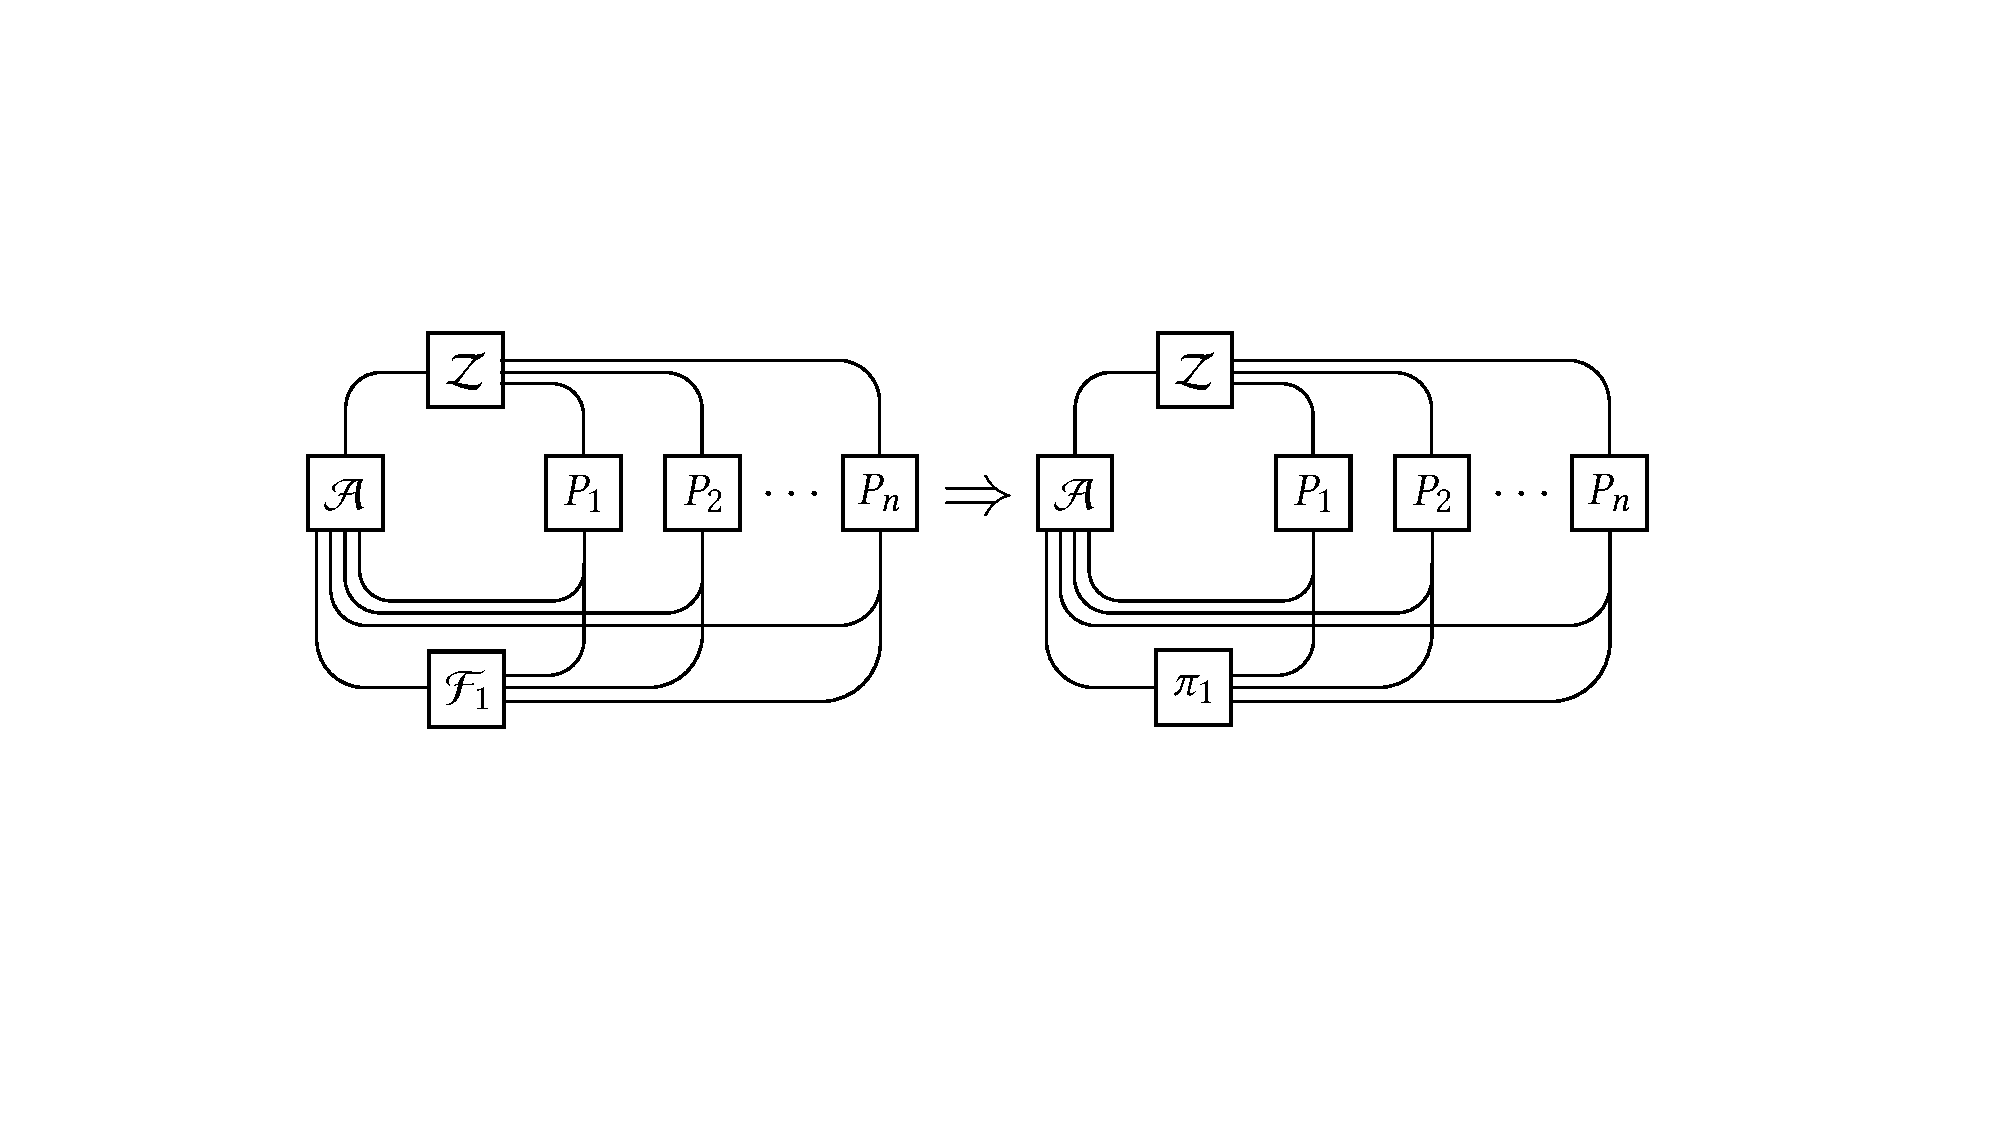
\includegraphics[width=\linewidth]{graphics/composition}
  \caption{UC protocol composition theorem.}
  \label{fig:uc-composition}
\end{figure}
\end{comment}
